%\VignetteIndexEntry{faoswsAupus: A package replicating the logic of the AUPUS
% statistical working system}
%\VignetteEngine{knitr::knitr}
\documentclass[nojss]{jss}
\usepackage{url}
\usepackage[sc]{mathpazo}
\usepackage{geometry}
\geometry{verbose,tmargin=2.5cm,bmargin=2.5cm,lmargin=2.5cm,rmargin=2.5cm}
\setcounter{secnumdepth}{2}
\setcounter{tocdepth}{2}
\usepackage{breakurl}
\usepackage{hyperref}
\usepackage[ruled, vlined]{algorithm2e}
\usepackage{mathtools}
\usepackage{draftwatermark}
\usepackage{float}
\usepackage{placeins}
\usepackage{mathrsfs}
\usepackage{multirow}
%% \usepackage{mathbbm}
\DeclareMathOperator{\sgn}{sgn}
\DeclareMathOperator*{\argmax}{\arg\!\max}

\title{\bf faoswsAupus: A package replicating the logic of the AUPUS
statistical working system}

\author{Joshua M. Browning, Michael. C. J. Kao\\ Food and Agriculture
    Organization \\ of the United Nations\\}

\Plainauthor{Joshua M. Browning, Michael. C. J. Kao}

\Plaintitle{faoswsAupus: A package replicating the logic of the AUPUS
statistical working system}

\Shorttitle{AUPUS Module}

\Abstract{ 

  This vignette provides a detailed description of the usage of
  functions in the \pkg{faoswsAupus} package. \\
  
}

\Keywords{AUPUS, Standardization}
\Plainkeywords{AUPUS, Standardization}

\Address{
  Joshua M. Browning and Michael. C. J. Kao\\
  Economics and Social Statistics Division (ESS)\\
  Economic and Social Development Department (ES)\\
  Food and Agriculture Organization of the United Nations (FAO)\\
  Viale delle Terme di Caracalla 00153 Rome, Italy\\
  E-mail: \email{joshua.browning@fao.org, michael.kao@fao.org}\\
  URL: \url{https://svn.fao.org/projects/SWS/RModules/faoswsAupus/}
}

\begin{document}



\section{Data Initialization}

First, we need to load the relevant packages:

\begin{knitrout}
\definecolor{shadecolor}{rgb}{0.969, 0.969, 0.969}\color{fgcolor}\begin{kframe}
\begin{alltt}
\hlkwd{library}\hlstd{(faoswsAupus)}
\hlkwd{library}\hlstd{(faosws)}
\hlkwd{library}\hlstd{(igraph)}
\hlkwd{library}\hlstd{(data.table)}
\end{alltt}
\end{kframe}
\end{knitrout}

This package comes with many functions for replicating the AUPUS and 
standardization procedures as well as several useful datasets.  The first we
will use is called 'US', and it contains an example of the data that is used
within this package.  There is also a variable called usAupusParam, and that
variable contains information about the US dataset.

\begin{knitrout}
\definecolor{shadecolor}{rgb}{0.969, 0.969, 0.969}\color{fgcolor}\begin{kframe}
\begin{alltt}
\hlkwd{is}\hlstd{(US)}
\end{alltt}
\begin{verbatim}
## [1] "list"   "vector"
\end{verbatim}
\begin{alltt}
\hlkwd{names}\hlstd{(US)}
\end{alltt}
\begin{verbatim}
## [1] "aupusData"          "inputData"          "ratioData"         
## [4] "shareData"          "balanceElementData" "itemInfoData"      
## [7] "populationData"     "extractionRateData"
\end{verbatim}
\begin{alltt}
\hlkwd{sapply}\hlstd{(US, class)}
\end{alltt}
\begin{verbatim}
##      aupusData    inputData    ratioData    shareData    balanceElementData
## [1,] "data.table" "data.table" "data.table" "data.table" "data.table"      
## [2,] "data.frame" "data.frame" "data.frame" "data.frame" "data.frame"      
##      itemInfoData populationData extractionRateData
## [1,] "data.table" "data.table"   "data.table"      
## [2,] "data.frame" "data.frame"   "data.frame"
\end{verbatim}
\begin{alltt}
\hlkwd{sapply}\hlstd{(US, dim)}
\end{alltt}
\begin{verbatim}
##      aupusData inputData ratioData shareData balanceElementData itemInfoData
## [1,]        15        10        15        10                 15            3
## [2,]        75         6        37         5                  4            3
##      populationData extractionRateData
## [1,]              5                 15
## [2,]              6                  5
\end{verbatim}
\begin{alltt}
\hlkwd{is}\hlstd{(usAupusParam)}
\end{alltt}
\begin{verbatim}
## [1] "list"   "vector"
\end{verbatim}
\begin{alltt}
\hlkwd{names}\hlstd{(usAupusParam)}
\end{alltt}
\begin{verbatim}
## [1] "areaCode"    "itemCode"    "elementCode" "year"        "keyNames"
\end{verbatim}
\end{kframe}
\end{knitrout}

Note: usually these values would be generated in the following manner:

\begin{knitrout}
\definecolor{shadecolor}{rgb}{0.969, 0.969, 0.969}\color{fgcolor}\begin{kframe}
\begin{alltt}
\hlkwd{GetTestEnvironment}\hlstd{(}
    \hlkwc{baseUrl} \hlstd{=} \hlstr{"https://hqlprswsas1.hq.un.fao.org:8181/sws"}\hlstd{,}
    \hlkwc{token} \hlstd{=} \hlstr{"66984d62-6add-4ad4-bdf3-5d8538bb2b70"}\hlstd{)}
\hlstd{usAupusParam} \hlkwb{=} \hlkwd{getAupusParameter}\hlstd{(}\hlkwc{areaCode} \hlstd{=} \hlstr{"231"}\hlstd{,} \hlkwc{assignGlobal} \hlstd{=} \hlnum{FALSE}\hlstd{,}
                                 \hlkwc{yearsToUse} \hlstd{=} \hlnum{2009}\hlopt{:}\hlnum{2013}\hlstd{)}
\hlstd{US} \hlkwb{=} \hlkwd{getAupusDataset}\hlstd{(}\hlkwc{aupusParam} \hlstd{= usAupusParam)}
\end{alltt}
\end{kframe}
\end{knitrout}

The GetTestEnvironment function from the faosws package sets up the right
variables in R for querying the SWS database, and the specific token I used
provides the necessary information for the AUPUS dataset.  The parameters and
data are then pulled from the SWS.  However, for this vignette, we'll just use
the data that already exists in this package.

We see that the US dataset contains 8 data.tables.  Let's look at a subset of
this data to more easily understand what we're working with.  First, let's
ensure we grab a meaningful subset of data.  The plotCommodityTree function
takes the shareData dataset and generates a plot for how the commodities are
related to one another.

\begin{knitrout}
\definecolor{shadecolor}{rgb}{0.969, 0.969, 0.969}\color{fgcolor}\begin{kframe}
\begin{alltt}
\hlkwd{plotCommodityTree}\hlstd{(US}\hlopt{$}\hlstd{shareData)}
\end{alltt}
\end{kframe}

{\centering 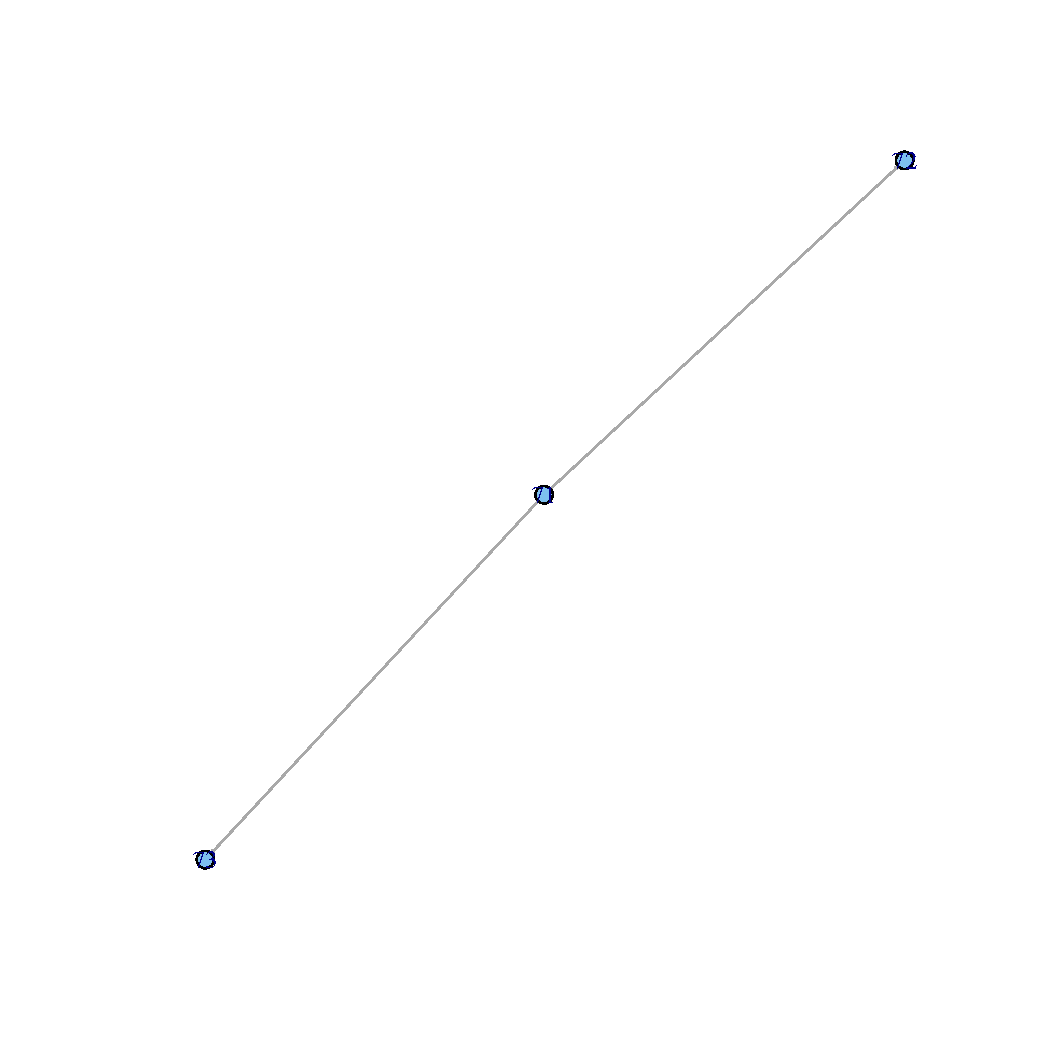
\includegraphics[width=\maxwidth]{figure/unnamed-chunk-3-1} 

}



\end{knitrout}

For simplicity, let's look at only commodities 71, 72, and 73.

\begin{knitrout}
\definecolor{shadecolor}{rgb}{0.969, 0.969, 0.969}\color{fgcolor}\begin{kframe}
\begin{alltt}
\hlstd{US} \hlkwb{=} \hlkwd{subsetAupus}\hlstd{(}\hlkwc{aupusData} \hlstd{= US,} \hlkwc{itemKeys} \hlstd{=} \hlkwd{c}\hlstd{(}\hlnum{71}\hlstd{,} \hlnum{72}\hlstd{,} \hlnum{73}\hlstd{),}
                 \hlkwc{aupusParam} \hlstd{= usAupusParam)}
\end{alltt}
\end{kframe}
\end{knitrout}

Now, we wish to work with this data in a network framework, and the package
contains a few functions to generate that framework:

\begin{knitrout}
\definecolor{shadecolor}{rgb}{0.969, 0.969, 0.969}\color{fgcolor}\begin{kframe}
\begin{alltt}
\hlstd{aupusNetwork} \hlkwb{=} \hlkwd{suaToNetworkRepresentation}\hlstd{(}\hlkwc{dataList} \hlstd{= US,}
                                          \hlkwc{aupusParam} \hlstd{= usAupusParam)}
\hlkwd{names}\hlstd{(aupusNetwork)}
\end{alltt}
\begin{verbatim}
## [1] "nodes" "edges"
\end{verbatim}
\begin{alltt}
\hlkwd{sapply}\hlstd{(aupusNetwork, class)}
\end{alltt}
\begin{verbatim}
##      nodes        edges       
## [1,] "data.table" "data.table"
## [2,] "data.frame" "data.frame"
\end{verbatim}
\begin{alltt}
\hlkwd{sapply}\hlstd{(aupusNetwork, dim)}
\end{alltt}
\begin{verbatim}
##      nodes edges
## [1,]    15    10
## [2,]   114     9
\end{verbatim}
\end{kframe}
\end{knitrout}

We see that now the data has been condensed down into two objects: nodes and
edges.  The nodes dataset has 15 rows (5 years times 3 commodities).
There are only 10 rows in the edges dataset, as there are only 2 edges times
5 years.  The nodes dataset is essentially the merged aupusData, itemInfoData,
ratioData, balanceElementData, and populationData from US, while the edges
dataset contains the datasets shareData, extractionRateData, and inputData from
US.  Here's our reduced network visualization:

\begin{knitrout}
\definecolor{shadecolor}{rgb}{0.969, 0.969, 0.969}\color{fgcolor}\begin{kframe}
\begin{alltt}
\hlkwd{plotCommodityTree}\hlstd{(US}\hlopt{$}\hlstd{shareData,} \hlkwc{edge.arrow.size} \hlstd{=} \hlnum{2}\hlstd{,} \hlkwc{vertex.size} \hlstd{=} \hlnum{25}\hlstd{)}
\hlstd{aupusNetwork}\hlopt{$}\hlstd{nodes[,} \hlkwd{.}\hlstd{(geographicAreaFS, timePointYearsSP, measuredItemFS)]}
\end{alltt}
\begin{verbatim}
##     geographicAreaFS timePointYearsSP measuredItemFS
##  1:              231             2009             71
##  2:              231             2010             71
##  3:              231             2011             71
##  4:              231             2012             71
##  5:              231             2013             71
##  6:              231             2009             72
##  7:              231             2010             72
##  8:              231             2011             72
##  9:              231             2012             72
## 10:              231             2013             72
## 11:              231             2009             73
## 12:              231             2010             73
## 13:              231             2011             73
## 14:              231             2012             73
## 15:              231             2013             73
\end{verbatim}
\begin{alltt}
\hlkwd{colnames}\hlstd{(aupusNetwork}\hlopt{$}\hlstd{nodes)[}\hlnum{1}\hlopt{:}\hlnum{10}\hlstd{]}
\end{alltt}
\begin{verbatim}
##  [1] "geographicAreaFS"                 "timePointYearsSP"                
##  [3] "measuredItemFS"                   "Value_measuredElementFS_11"      
##  [5] "flagFaostat_measuredElementFS_11" "Value_measuredElementFS_21"      
##  [7] "flagFaostat_measuredElementFS_21" "Value_measuredElementFS_31"      
##  [9] "flagFaostat_measuredElementFS_31" "Value_measuredElementFS_41"
\end{verbatim}
\begin{alltt}
\hlstd{aupusNetwork}\hlopt{$}\hlstd{edges[,} \hlkwd{.}\hlstd{(geographicAreaFS, timePointYearsSP,}
                       \hlstd{measuredItemParentFS, measuredItemChildFS)]}
\end{alltt}
\begin{verbatim}
##     geographicAreaFS timePointYearsSP measuredItemParentFS measuredItemChildFS
##  1:              231             2009                   71                  72
##  2:              231             2010                   71                  72
##  3:              231             2011                   71                  72
##  4:              231             2012                   71                  72
##  5:              231             2013                   71                  72
##  6:              231             2009                   71                  73
##  7:              231             2010                   71                  73
##  8:              231             2011                   71                  73
##  9:              231             2012                   71                  73
## 10:              231             2013                   71                  73
\end{verbatim}
\begin{alltt}
\hlkwd{colnames}\hlstd{(aupusNetwork}\hlopt{$}\hlstd{edges)}
\end{alltt}
\begin{verbatim}
## [1] "geographicAreaFS"       "measuredItemParentFS"   "measuredItemChildFS"   
## [4] "timePointYearsSP"       "Value_share"            "Value_extraction"      
## [7] "flagFaostat_extraction" "Value_input"            "flagFaostat_input"
\end{verbatim}
\end{kframe}

{\centering 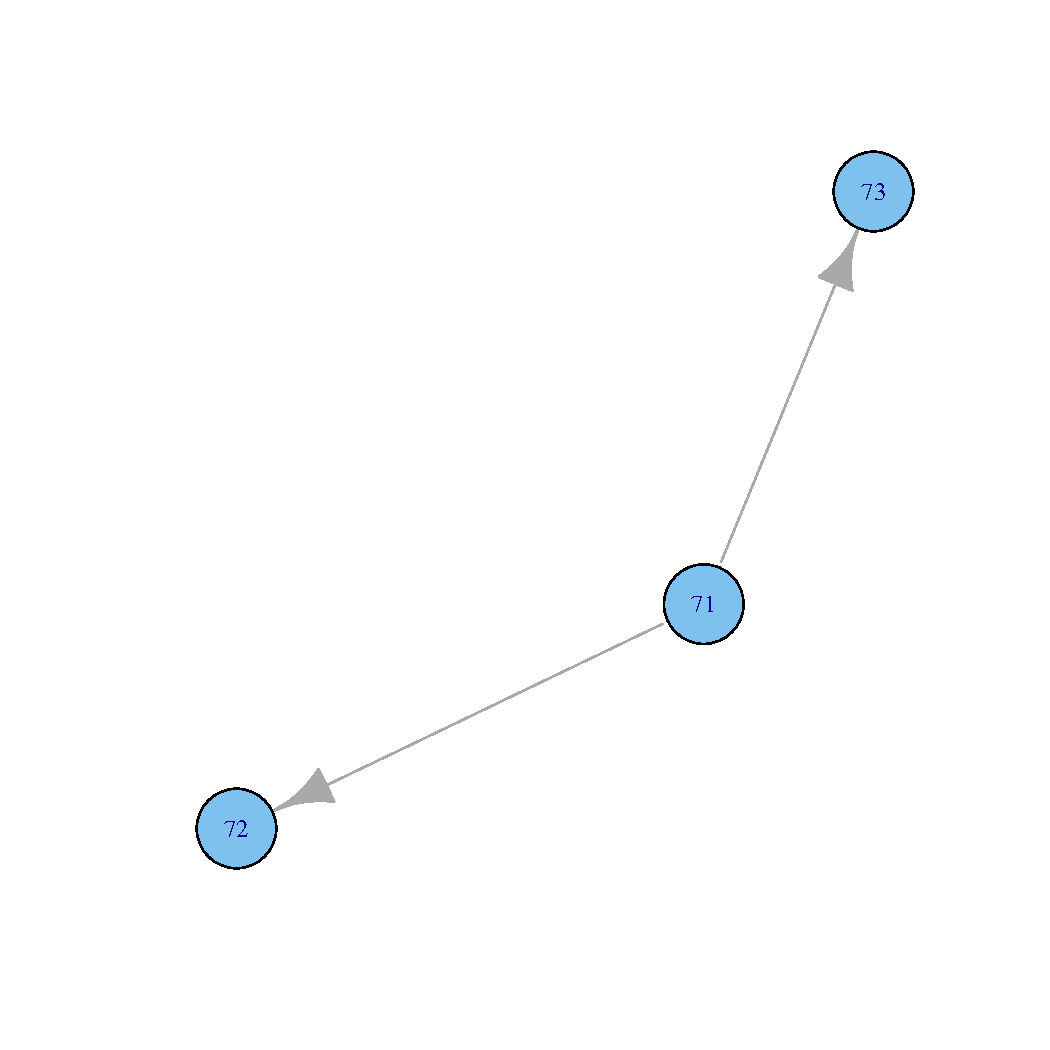
\includegraphics[width=\maxwidth]{figure/unnamed-chunk-6-1} 

}



\end{knitrout}

\section{AUPUS}

The entire AUPUS procedure is encapsulated in one function: Aupus.  However,
let's look at some of the functions called within this main function to
understand how the process works.  First, we have to set up some of the things
as done by the Aupus function:

\begin{knitrout}
\definecolor{shadecolor}{rgb}{0.969, 0.969, 0.969}\color{fgcolor}\begin{kframe}
\begin{alltt}
\hlstd{nodes} \hlkwb{=} \hlstd{aupusNetwork}\hlopt{$}\hlstd{nodes}
\hlstd{edges} \hlkwb{=} \hlstd{aupusNetwork}\hlopt{$}\hlstd{edges}
\hlstd{nodes} \hlkwb{=} \hlkwd{coerceColumnTypes}\hlstd{(}\hlkwc{aupusParam} \hlstd{= usAupusParam,} \hlkwc{data} \hlstd{= nodes)}
\hlstd{edges} \hlkwb{=} \hlkwd{coerceColumnTypes}\hlstd{(}\hlkwc{aupusParam} \hlstd{= usAupusParam,} \hlkwc{data} \hlstd{= edges)}
\hlstd{from} \hlkwb{=} \hlstd{usAupusParam}\hlopt{$}\hlstd{keyNames}\hlopt{$}\hlstd{itemParentName}
\hlstd{to} \hlkwb{=} \hlstd{usAupusParam}\hlopt{$}\hlstd{keyNames}\hlopt{$}\hlstd{itemChildName}
\hlstd{processingLevelData} \hlkwb{=} \hlstd{edges[,} \hlkwd{findProcessingLevel}\hlstd{(.SD,} \hlkwc{from} \hlstd{= from,}
    \hlkwc{to} \hlstd{= to,} \hlkwc{aupusParam} \hlstd{= usAupusParam),}
    \hlkwc{by} \hlstd{=} \hlkwd{c}\hlstd{(usAupusParam}\hlopt{$}\hlstd{keyNames}\hlopt{$}\hlstd{areaName, usAupusParam}\hlopt{$}\hlstd{keyNames}\hlopt{$}\hlstd{yearName)]}
\hlkwd{setkeyv}\hlstd{(processingLevelData,} \hlkwd{key}\hlstd{(nodes))}
\hlkwd{invisible}\hlstd{(nodes[processingLevelData,} \hlkwd{`:=`}\hlstd{(processingLevel, i.processingLevel)])}
\hlkwd{invisible}\hlstd{(nodes[}\hlkwd{is.na}\hlstd{(processingLevel), processingLevel} \hlkwb{:=} \hlnum{0}\hlstd{])}
\hlstd{nodes[,} \hlkwd{c}\hlstd{(}\hlkwd{key}\hlstd{(nodes),} \hlstr{"processingLevel"}\hlstd{),} \hlkwc{with} \hlstd{=} \hlnum{FALSE}\hlstd{]}
\end{alltt}
\begin{verbatim}
##     geographicAreaFS measuredItemFS timePointYearsSP processingLevel
##  1:              231             71             2009               0
##  2:              231             71             2010               0
##  3:              231             71             2011               0
##  4:              231             71             2012               0
##  5:              231             71             2013               0
##  6:              231             72             2009               1
##  7:              231             72             2010               1
##  8:              231             72             2011               1
##  9:              231             72             2012               1
## 10:              231             72             2013               1
## 11:              231             73             2009               1
## 12:              231             73             2010               1
## 13:              231             73             2011               1
## 14:              231             73             2012               1
## 15:              231             73             2013               1
\end{verbatim}
\end{kframe}
\end{knitrout}

The processing level function above uses functions from the \pkg{igraph}
package to determine the ``processing level.''  This value indicates the order
in which a particular node is processed: nodes at level 0 have no
inputs/dependencies/children, and thus they can be processed immediately.  Once
level 0 nodes have been processed, we have the data necessary for processing
their parents, and these are nodes with processing level 1.  Aggregation
continues until all processing levels have been processed.

Our example is simple: 72 and 73 are children of 71, and so 71 must first be
processed before we process 72 and 73.  Thus, 71 is processingLevel = 0 and
72 and 73 have processingLevel = 1.

At each level, there are three main processes that are performed:
\begin{enumerate}
    \item The main AUPUS module is ran on each node.  This module computes each
    individual element following the logic of the old system.
    \item The edges of the graph are updated.
    \item The inputs from processing are updated.
\end{enumerate}

\subsection{Main AUPUS Module}

The main function here is calculateAupusElements.  This function calls all of
the individual element calculation functions.  Each element function has it's
own calculation, and is documented within it's help page.  However, we'll show
an example for a few of the functions.  First, though, note that we must subset
the AUPUS data: we only want to process the commodities at the lowest
processing level right now:

\begin{knitrout}
\definecolor{shadecolor}{rgb}{0.969, 0.969, 0.969}\color{fgcolor}\begin{kframe}
\begin{alltt}
\hlstd{toProcess} \hlkwb{=} \hlstd{nodes[processingLevel} \hlopt{==} \hlnum{0}\hlstd{, ]}
\end{alltt}
\end{kframe}
\end{knitrout}

Ok, now let's compute element 11:

\begin{knitrout}
\definecolor{shadecolor}{rgb}{0.969, 0.969, 0.969}\color{fgcolor}\begin{kframe}
\begin{alltt}
\hlstd{toProcess[, Value_measuredElementFS_11]}
\end{alltt}
\begin{verbatim}
## [1] 12000 23000 20000 20000 20000
\end{verbatim}
\begin{alltt}
\hlstd{toProcess[, Value_measuredElementFS_161]}
\end{alltt}
\begin{verbatim}
## [1] NA NA NA NA NA
\end{verbatim}
\begin{alltt}
\hlstd{toProcess[, flagFaostat_measuredElementFS_11]}
\end{alltt}
\begin{verbatim}
## [1] ""  ""  ""  "T" "T"
\end{verbatim}
\begin{alltt}
\hlkwd{calculateEle11}\hlstd{(}\hlkwc{data} \hlstd{= toProcess,} \hlkwc{aupusParam} \hlstd{= usAupusParam)}
\end{alltt}
\begin{verbatim}
## integer(0)
\end{verbatim}
\begin{alltt}
\hlstd{toProcess[, Value_measuredElementFS_11]}
\end{alltt}
\begin{verbatim}
## [1] 12000 23000 20000 20000 20000
\end{verbatim}
\begin{alltt}
\hlstd{toProcess[, flagFaostat_measuredElementFS_11]}
\end{alltt}
\begin{verbatim}
## [1] ""  ""  ""  "T" "T"
\end{verbatim}
\end{kframe}
\end{knitrout}

Element 11 is called ``Initial Existence'' and thus it is set to
``Final Existence'' (element 161) from the previous year, if that value exists
and if element 11 is currently missing.  In this case, all of element 161's
values are missing and thus no updating occurs.  Let's continue processing some
elements:

\begin{knitrout}
\definecolor{shadecolor}{rgb}{0.969, 0.969, 0.969}\color{fgcolor}\begin{kframe}
\begin{alltt}
\hlkwd{calculateEle21}\hlstd{(}\hlkwc{data} \hlstd{= toProcess,} \hlkwc{aupusParam} \hlstd{= usAupusParam)}
\end{alltt}
\begin{verbatim}
## integer(0)
\end{verbatim}
\begin{alltt}
\hlkwd{calculateEle41}\hlstd{(}\hlkwc{data} \hlstd{= toProcess,} \hlkwc{aupusParam} \hlstd{= usAupusParam)}
\end{alltt}
\begin{verbatim}
## integer(0)
\end{verbatim}
\begin{alltt}
\hlkwd{calculateEle51}\hlstd{(}\hlkwc{data} \hlstd{= toProcess,} \hlkwc{aupusParam} \hlstd{= usAupusParam)}
\end{alltt}
\begin{verbatim}
## integer(0)
\end{verbatim}
\begin{alltt}
\hlkwd{calculateEle314151}\hlstd{(}\hlkwc{data} \hlstd{= toProcess,} \hlkwc{aupusParam} \hlstd{= usAupusParam)}
\end{alltt}
\begin{verbatim}
## [[1]]
## integer(0)
## 
## [[2]]
## integer(0)
\end{verbatim}
\begin{alltt}
\hlkwd{calculateEle63}\hlstd{(}\hlkwc{data} \hlstd{= toProcess,} \hlkwc{aupusParam} \hlstd{= usAupusParam)}
\end{alltt}
\begin{verbatim}
## [[1]]
## [1] 1 2 3 4 5
## 
## [[2]]
## integer(0)
\end{verbatim}
\begin{alltt}
\hlkwd{calculateEle71}\hlstd{(}\hlkwc{data} \hlstd{= toProcess,} \hlkwc{aupusParam} \hlstd{= usAupusParam)}
\end{alltt}
\begin{verbatim}
## [[1]]
## integer(0)
## 
## [[2]]
## integer(0)
\end{verbatim}
\begin{alltt}
\hlkwd{calculateEle93}\hlstd{(}\hlkwc{data} \hlstd{= toProcess,} \hlkwc{aupusParam} \hlstd{= usAupusParam)}
\end{alltt}
\begin{verbatim}
## [[1]]
## [1] 1 2 3 4 5
## 
## [[2]]
## integer(0)
\end{verbatim}
\begin{alltt}
\hlkwd{calculateTotalSupply}\hlstd{(}\hlkwc{data} \hlstd{= toProcess,} \hlkwc{aupusParam} \hlstd{= usAupusParam)}
\hlkwd{tail}\hlstd{(}\hlkwd{colnames}\hlstd{(toProcess))}
\end{alltt}
\begin{verbatim}
## [1] "Value_balanceElement" "Value_population_11"  "Value_population_21" 
## [4] "processingLevel"      "newSummation"         "TOTAL_SUPPLY"
\end{verbatim}
\begin{alltt}
\hlstd{toProcess}\hlopt{$}\hlstd{TOTAL_SUPPLY}
\end{alltt}
\begin{verbatim}
## [1] 297711 309126 331715 347403 365818
\end{verbatim}
\end{kframe}
\end{knitrout}

Each of the calculateEleXX functions above calculates updated values for each
element and returns a vector of list of vectors with indices.  These indices
represent the rows that were updated in the computation of this element.  The
last function, calculateTotalSupply, returns nothing but adds an additional
column to the toProcess data.table.  This column, TOTAL\_SUPPLY, represents the
total supply for this commodity.  Now, we can proceed with computing other
elements.  Some elements, such as 101, 111, 121, 131, and 141 use total supply
to fill in their values:

\begin{knitrout}
\definecolor{shadecolor}{rgb}{0.969, 0.969, 0.969}\color{fgcolor}\begin{kframe}
\begin{alltt}
\hlkwd{calculateEle101}\hlstd{(}\hlkwc{stotal} \hlstd{=} \hlstr{"TOTAL_SUPPLY"}\hlstd{,} \hlkwc{data} \hlstd{= toProcess,}
                \hlkwc{aupusParam} \hlstd{= usAupusParam)}
\end{alltt}
\begin{verbatim}
## integer(0)
\end{verbatim}
\begin{alltt}
\hlkwd{calculateEle111}\hlstd{(}\hlkwc{stotal} \hlstd{=} \hlstr{"TOTAL_SUPPLY"}\hlstd{,} \hlkwc{data} \hlstd{= toProcess,}
                \hlkwc{aupusParam} \hlstd{= usAupusParam)}
\end{alltt}
\begin{verbatim}
## [[1]]
## integer(0)
## 
## [[2]]
## integer(0)
\end{verbatim}
\begin{alltt}
\hlkwd{calculateEle121}\hlstd{(}\hlkwc{stotal} \hlstd{=} \hlstr{"TOTAL_SUPPLY"}\hlstd{,} \hlkwc{data} \hlstd{= toProcess,}
                \hlkwc{aupusParam} \hlstd{= usAupusParam)}
\end{alltt}
\begin{verbatim}
## integer(0)
\end{verbatim}
\begin{alltt}
\hlkwd{calculateEle131}\hlstd{(}\hlkwc{stotal} \hlstd{=} \hlstr{"TOTAL_SUPPLY"}\hlstd{,} \hlkwc{data} \hlstd{= toProcess,}
                \hlkwc{aupusParam} \hlstd{= usAupusParam)}
\end{alltt}
\begin{verbatim}
## integer(0)
\end{verbatim}
\begin{alltt}
\hlkwd{calculateEle141}\hlstd{(}\hlkwc{stotal} \hlstd{=} \hlstr{"TOTAL_SUPPLY"}\hlstd{,} \hlkwc{data} \hlstd{= toProcess,}
                \hlkwc{aupusParam} \hlstd{= usAupusParam)}
\end{alltt}
\begin{verbatim}
## [1] 1 2 3 4 5
\end{verbatim}
\begin{alltt}
\hlkwd{calculateEle144}\hlstd{(}\hlkwc{population11Num} \hlstd{=} \hlstr{"Value_population_11"}\hlstd{,}
                \hlkwc{data} \hlstd{= toProcess,} \hlkwc{aupusParam} \hlstd{= usAupusParam)}
\end{alltt}
\begin{verbatim}
## integer(0)
\end{verbatim}
\begin{alltt}
\hlkwd{calculateEle151}\hlstd{(}\hlkwc{stotal} \hlstd{=} \hlstr{"TOTAL_SUPPLY"}\hlstd{,} \hlkwc{data} \hlstd{= toProcess,}
                \hlkwc{aupusParam} \hlstd{= usAupusParam)}
\end{alltt}
\begin{verbatim}
## integer(0)
\end{verbatim}
\begin{alltt}
\hlkwd{calculateEle161}\hlstd{(}\hlkwc{data} \hlstd{= toProcess,} \hlkwc{aupusParam} \hlstd{= usAupusParam)}
\end{alltt}
\begin{verbatim}
## integer(0)
\end{verbatim}
\begin{alltt}
\hlkwd{calculateEle171}\hlstd{(}\hlkwc{data} \hlstd{= toProcess,} \hlkwc{aupusParam} \hlstd{= usAupusParam)}
\end{alltt}
\begin{verbatim}
## integer(0)
\end{verbatim}
\begin{alltt}
\hlkwd{calculateEle174}\hlstd{(}\hlkwc{population11Num} \hlstd{=} \hlstr{"Value_population_11"}\hlstd{,}
                                   \hlkwc{data} \hlstd{= toProcess,}
                                   \hlkwc{aupusParam} \hlstd{= usAupusParam)}
\end{alltt}
\begin{verbatim}
## integer(0)
\end{verbatim}
\end{kframe}
\end{knitrout}

Once we've computed element 141, we can compute nutritive values: calories,
proteins, and fats.  These are based on ratios provided in the database (to
convert quantity into these values).

\begin{knitrout}
\definecolor{shadecolor}{rgb}{0.969, 0.969, 0.969}\color{fgcolor}\begin{kframe}
\begin{alltt}
\hlkwd{calculateTotalNutritive}\hlstd{(}\hlkwc{ratioNum} \hlstd{=} \hlstr{"Ratio_measuredElementFS_261"}\hlstd{,}
                            \hlkwc{elementNum} \hlstd{=} \hlnum{261}\hlstd{,} \hlkwc{data} \hlstd{= toProcess,}
                            \hlkwc{aupusParam} \hlstd{= usAupusParam)}
\end{alltt}
\begin{verbatim}
## integer(0)
\end{verbatim}
\begin{alltt}
\hlkwd{calculateDailyNutritive}\hlstd{(}\hlkwc{population11Num} \hlstd{=} \hlstr{"Value_population_11"}\hlstd{,}
                        \hlkwc{population21Num} \hlstd{=} \hlstr{"Value_population_21"}\hlstd{,}
                        \hlkwc{dailyElement} \hlstd{=} \hlnum{264}\hlstd{,} \hlkwc{totalElement} \hlstd{=} \hlnum{261}\hlstd{,}
                        \hlkwc{data} \hlstd{= toProcess,} \hlkwc{aupusParam} \hlstd{= usAupusParam)}
\end{alltt}
\begin{verbatim}
## integer(0)
\end{verbatim}
\begin{alltt}
\hlkwd{calculateTotalNutritive}\hlstd{(}\hlkwc{ratioNum} \hlstd{=} \hlstr{"Ratio_measuredElementFS_271"}\hlstd{,}
                            \hlkwc{elementNum} \hlstd{=} \hlnum{271}\hlstd{,} \hlkwc{data} \hlstd{= toProcess,}
                            \hlkwc{aupusParam} \hlstd{= usAupusParam)}
\end{alltt}
\begin{verbatim}
## integer(0)
\end{verbatim}
\begin{alltt}
\hlkwd{calculateDailyNutritive}\hlstd{(}\hlkwc{population11Num} \hlstd{=} \hlstr{"Value_population_11"}\hlstd{,}
                        \hlkwc{population21Num} \hlstd{=} \hlstr{"Value_population_21"}\hlstd{,}
                        \hlkwc{dailyElement} \hlstd{=} \hlnum{274}\hlstd{,} \hlkwc{totalElement} \hlstd{=} \hlnum{271}\hlstd{,}
                        \hlkwc{data} \hlstd{= toProcess,} \hlkwc{aupusParam} \hlstd{= usAupusParam)}
\end{alltt}
\begin{verbatim}
## integer(0)
\end{verbatim}
\begin{alltt}
\hlkwd{calculateTotalNutritive}\hlstd{(}\hlkwc{ratioNum} \hlstd{=} \hlstr{"Ratio_measuredElementFS_281"}\hlstd{,}
                            \hlkwc{elementNum} \hlstd{=} \hlnum{281}\hlstd{,} \hlkwc{data} \hlstd{= toProcess,}
                            \hlkwc{aupusParam} \hlstd{= usAupusParam)}
\end{alltt}
\begin{verbatim}
## integer(0)
\end{verbatim}
\begin{alltt}
\hlkwd{calculateDailyNutritive}\hlstd{(}\hlkwc{population11Num} \hlstd{=} \hlstr{"Value_population_11"}\hlstd{,}
                        \hlkwc{population21Num} \hlstd{=} \hlstr{"Value_population_21"}\hlstd{,}
                        \hlkwc{dailyElement} \hlstd{=} \hlnum{284}\hlstd{,} \hlkwc{totalElement} \hlstd{=} \hlnum{281}\hlstd{,}
                        \hlkwc{data} \hlstd{= toProcess,} \hlkwc{aupusParam} \hlstd{= usAupusParam)}
\end{alltt}
\begin{verbatim}
## integer(0)
\end{verbatim}
\end{kframe}
\end{knitrout}

We now need to calculate two remaining elements (541 and 546, containing final
and total demand) and then we can balance.

\begin{knitrout}
\definecolor{shadecolor}{rgb}{0.969, 0.969, 0.969}\color{fgcolor}\begin{kframe}
\begin{alltt}
\hlkwd{calculateEle541}\hlstd{(}\hlkwc{data} \hlstd{= toProcess,} \hlkwc{aupusParam} \hlstd{= usAupusParam)}
\end{alltt}
\begin{verbatim}
## integer(0)
\end{verbatim}
\begin{alltt}
\hlkwd{calculateEle546}\hlstd{(}\hlkwc{data} \hlstd{= toProcess,} \hlkwc{aupusParam} \hlstd{= usAupusParam)}
\end{alltt}
\begin{verbatim}
## integer(0)
\end{verbatim}
\begin{alltt}
\hlkwd{calculateTotalUtilization}\hlstd{(}\hlkwc{data} \hlstd{= toProcess,} \hlkwc{aupusParam} \hlstd{= usAupusParam)}
\hlkwd{calculateBalance}\hlstd{(}\hlkwc{supply} \hlstd{=} \hlstr{"TOTAL_SUPPLY"}\hlstd{,} \hlkwc{utilization} \hlstd{=} \hlstr{"TOTAL_UTILIZATION"}\hlstd{,}
                 \hlkwc{data} \hlstd{= toProcess,} \hlkwc{aupusParam} \hlstd{= usAupusParam)}
\end{alltt}
\begin{verbatim}
## integer(0)
\end{verbatim}
\begin{alltt}
\hlkwd{tail}\hlstd{(}\hlkwd{colnames}\hlstd{(toProcess))}
\end{alltt}
\begin{verbatim}
## [1] "Value_measuredElementFS_542" "Value_measuredElementFS_543"
## [3] "Value_measuredElementFS_544" "Value_measuredElementFS_545"
## [5] "TOTAL_UTILIZATION"           "BALANCE"
\end{verbatim}
\end{kframe}
\end{knitrout}

Now, we have the TOTAL\_SUPPLY, TOTAL\_UTILIZATION, and BALANCE values.

\subsection{Update Edges}

The second step in the AUPUS procedure is to update the edges of the commodity
network.  In this step, we're updating the extraction rates and the input from
processing values on the edges data.table with the values from the nodes
table.  Note: the 131 element represents the input from processing value, and
the 41 element has extraction rates.

\begin{knitrout}
\definecolor{shadecolor}{rgb}{0.969, 0.969, 0.969}\color{fgcolor}\begin{kframe}
\begin{alltt}
\hlstd{toProcess[,} \hlkwd{c}\hlstd{(}\hlstr{"timePointYearsSP"}\hlstd{,} \hlstr{"Value_measuredElementFS_131"}\hlstd{,}
              \hlstr{"Value_measuredElementFS_41"}\hlstd{),} \hlkwc{with} \hlstd{= F]}
\end{alltt}
\begin{verbatim}
##    timePointYearsSP Value_measuredElementFS_131 Value_measuredElementFS_41
## 1:             2009                       83800                   17418.12
## 2:             2010                       83800                   17601.64
## 3:             2011                       84000                   16408.66
## 4:             2012                       84000                   17574.18
## 5:             2013                       84000                   17314.47
\end{verbatim}
\begin{alltt}
\hlstd{edges[,} \hlkwd{c}\hlstd{(}\hlstr{"timePointYearsSP"}\hlstd{,} \hlstr{"measuredItemChildFS"}\hlstd{,} \hlstr{"Value_share"}\hlstd{,}
          \hlstr{"Value_input"}\hlstd{,} \hlstr{"Value_extraction"}\hlstd{),} \hlkwc{with} \hlstd{=} \hlnum{FALSE}\hlstd{]}
\end{alltt}
\begin{verbatim}
##     timePointYearsSP measuredItemChildFS Value_share Value_input
##  1:             2009                  72         100       83800
##  2:             2010                  72         100       83800
##  3:             2011                  72         100       84000
##  4:             2012                  72         100       84000
##  5:             2013                  72         100       84000
##  6:             2009                  73         100       83800
##  7:             2010                  73         100       83800
##  8:             2011                  73         100       84000
##  9:             2012                  73         100       84000
## 10:             2013                  73         100       84000
##     Value_extraction
##  1:             8000
##  2:             8000
##  3:             8000
##  4:             8000
##  5:             8000
##  6:             1600
##  7:             1600
##  8:             1600
##  9:             1600
## 10:             1600
\end{verbatim}
\begin{alltt}
\hlkwd{updateEdges}\hlstd{(}\hlkwc{nodes} \hlstd{= toProcess,} \hlkwc{edges} \hlstd{= edges,} \hlkwc{aupusParam} \hlstd{= usAupusParam)}
\hlstd{edges[,} \hlkwd{c}\hlstd{(}\hlstr{"timePointYearsSP"}\hlstd{,} \hlstr{"measuredItemChildFS"}\hlstd{,} \hlstr{"Value_share"}\hlstd{,}
          \hlstr{"Value_input"}\hlstd{,} \hlstr{"Value_extraction"}\hlstd{),} \hlkwc{with} \hlstd{=} \hlnum{FALSE}\hlstd{]}
\end{alltt}
\begin{verbatim}
##     timePointYearsSP measuredItemChildFS Value_share Value_input
##  1:             2009                  72         100       83800
##  2:             2010                  72         100       83800
##  3:             2011                  72         100       84000
##  4:             2012                  72         100       84000
##  5:             2013                  72         100       84000
##  6:             2009                  73         100       83800
##  7:             2010                  73         100       83800
##  8:             2011                  73         100       84000
##  9:             2012                  73         100       84000
## 10:             2013                  73         100       84000
##     Value_extraction
##  1:         17418.12
##  2:         17601.64
##  3:         16408.66
##  4:         17574.18
##  5:         17314.47
##  6:         17418.12
##  7:         17601.64
##  8:         16408.66
##  9:         17574.18
## 10:         17314.47
\end{verbatim}
\end{kframe}
\end{knitrout}

The Value\_input column of edges is updated (in theory) to reflect the amount
of the parent commodity flowing to the child.  In this case, the original
values for inputs from processing were already correct, and so nothing is
changed with them.  However, the extraction rates are different, and those
values are changed on the edges table (updated to reflect the nodes table).

\subsection{Update Inputs from Processing}

In this step, the data from the edges data.table is passed to the nodes
data.table at the next processing level.













